%\documentclass[compress]{beamer}
\documentclass[8pt,xcolor=dvipnames]{beamer}

%-----------------------------------------------------------
% PACKAGES

%\usepackage[latin1]{inputenc}
\mode<presentation>

%\usepackage[T1]{fontenc}  
%\usetheme{Warsaw}
\usetheme{Frankfurt}
\definecolor{maroon}{RGB}{80, 0.0, 0.0}
\usecolortheme[named=maroon]{structure}
\useoutertheme[subsection=false]{miniframes}
\usepackage{etoolbox}
\makeatletter
\patchcmd{\slideentry}{\advance\beamer@xpos by1\relax}{}{}{}
\def\beamer@subsectionentry#1#2#3#4#5{\advance\beamer@xpos by1\relax}%
\makeatother

%\setbeamercolor{block title}{bg=red!30,fg=black}

\usepackage{graphicx}
%\usepackage[section]{placeins} % force � mettre l'image o� on veut
%\usepackage{float} %utiliser H pour forcer � mettre l'image o� on veut
\usepackage{lscape} %utilisation du mode paysage
%\usepackage{pslatex}
\usepackage{url}
\usepackage{subfigure}

\usepackage{graphicx}
\usepackage{tabls}
\usepackage{afterpage}

\usepackage{ocgx2}
\usepackage[]{media9}
%\usepackage{multimedia}

\usepackage{amsthm}
\usepackage{amssymb}
\usepackage{amsmath}
\usepackage{amsfonts}
\usepackage{amstext}
\usepackage{amsbsy}
\usepackage{mathbbol} 
\usepackage{mathrsfs}

\usepackage{epsfig}
%\usepackage{epsfig}
%\usepackage{cites}
\usepackage{epsf}
\usepackage{array}
\usepackage{color}
\usepackage{pdfpages}
\usepackage{cancel}

\usepackage{tikz}
\usepackage{colortbl}
%\usepackage{booktabs}
\usepackage{multicol}
\usepackage{caption}

%-----------------------------------------------------------
% NEW  DEFINITIONS
%
%=================================================================================================
% new commands
% +++++++++++++++++++++++++++++++++++++++++++++++++++++++++++++++++++++++++++++++++++++++++++++++++
\newcommand{\nc}{\newcommand}
%
% Ways of grouping things
%
\newcommand{\bracket}[1]{\left[ #1 \right]}
\newcommand{\bracet}[1]{\left\{ #1 \right\}}
\newcommand{\fn}[1]{\left( #1 \right)}
\newcommand{\ave}[1]{\left\langle #1 \right\rangle}
%
% Derivative forms
% 
\newcommand{\dx}[1]{\,d#1}
\newcommand{\dxdy}[2]{\frac{\partial #1}{\partial #2}}
\newcommand{\dxdt}[1]{\frac{\partial #1}{\partial t}}
\newcommand{\dxdz}[1]{\frac{\partial #1}{\partial z}}
\newcommand{\dfdt}[1]{\frac{\partial}{\partial t} \fn{#1}}
\newcommand{\dfdz}[1]{\frac{\partial}{\partial z} \fn{#1}}
\newcommand{\ddt}[1]{\frac{\partial}{\partial t} #1}
\newcommand{\ddz}[1]{\frac{\partial}{\partial z} #1}
\newcommand{\dd}[2]{\frac{\partial}{\partial #1} #2}
\newcommand{\ddx}[1]{\frac{\partial}{\partial x} #1}
\newcommand{\ddy}[1]{\frac{\partial}{\partial y} #1}
%
% Vector forms
%
%\renewcommand{\vec}[1]{\ensuremath{\stackrel{\rightarrow}{#1}}}
%\renewcommand{\div}{\ensuremath{\vec{\nabla} \cdot}}
%\newcommand{\grad}{\ensuremath{\vec{\nabla}}}

\renewcommand{\div}{\vec{\nabla}\! \cdot \!}
\newcommand{\grad}{\vec{\nabla}}
\newcommand{\oa}[1]{\fn{\frac{1}{3}\hat{\Omega}\!\cdot\!\overrightarrow{A_{#1}}}}

%
% Equation beginnings and endings
%
\newcommand{\bea}{\begin{eqnarray}}
\newcommand{\eea}{\end{eqnarray}}
\newcommand{\be}{\begin{equation*}}
\newcommand{\ee}{\end{equation*}}
\newcommand{\beas}{\begin{eqnarray*}}
\newcommand{\eeas}{\end{eqnarray*}}
\newcommand{\bdm}{\begin{displaymath}}
\newcommand{\edm}{\end{displaymath}}
%
% Equation punctuation
% 
\newcommand{\pec}{\hspace{0.25in},}
\newcommand{\pep}{\hspace{0.25in}.}
\newcommand{\pev}{\hspace{0.25in}}
%
% Equation labels and references, figure references, table references
% 
\newcommand{\LEQ}[1]{\label{eq:#1}}
\newcommand{\EQ}[1]{Eq.~(\ref{eq:#1})}
\newcommand{\EQS}[1]{Eqs.~(\ref{eq:#1})}
\newcommand{\REQ}[1]{\ref{eq:#1}}
\newcommand{\LFI}[1]{\label{fi:#1}}
\newcommand{\FI}[1]{Fig.~\ref{fi:#1}}
\newcommand{\RFI}[1]{\ref{fi:#1}}
\newcommand{\LTA}[1]{\label{ta:#1}}
\newcommand{\TA}[1]{Table~\ref{ta:#1}}
\newcommand{\RTA}[1]{\ref{ta:#1}}

%
% List beginnings and endings
% 
\newcommand{\bl}{\bss\begin{itemize}}
\newcommand{\el}{\vspace{-.5\baselineskip}\end{itemize}\ess}
\newcommand{\benu}{\bss\begin{enumerate}}
\newcommand{\eenu}{\vspace{-.5\baselineskip}\end{enumerate}\ess}
%
% Figure and table beginnings and endings
% 
\newcommand{\bfg}{\begin{figure}}
\newcommand{\efg}{\end{figure}}
\newcommand{\bt}{\begin{table}}
\newcommand{\et}{\end{table}}
%
% Tabular and center beginnings and endings
% 
\newcommand{\bc}{\begin{center}}
\newcommand{\ec}{\end{center}}
\newcommand{\btb}{\begin{center}\begin{tabular}}
\newcommand{\etb}{\end{tabular}\end{center}}
%
% Single space command
% 
%\newcommand{\bss}{\begin{singlespace}}
%\newcommand{\ess}{\end{singlespace}}
\newcommand{\bss}{\singlespacing}
\newcommand{\ess}{\doublespacing}
%
%---New environment "arbspace". (modeled after singlespace environment
%                                in Doublespace.sty)
%   The baselinestretch only takes effect at a size change, so do one.
% 
\def\arbspace#1{\def\baselinestretch{#1}\@normalsize}
\def\endarbspace{}
\newcommand{\bas}{\begin{arbspace}}
\newcommand{\eas}{\end{arbspace}}
%
% An explanation for a function
%
\newcommand{\explain}[1]{\mbox{\hspace{2em} #1}}
%
% Quick commands for symbols
%  
\newcommand{\half}{\frac{1}{2}}
\newcommand{\third}{\frac{1}{3}}
\newcommand{\twothird}{\frac{2}{3}}
\newcommand{\fourth}{\frac{1}{4}}
\newcommand{\mdot}{\dot{m}}
\newcommand{\ten}[1]{\times 10^{#1}\,}
\newcommand{\cL}{{\cal L}}
\newcommand{\cD}{{\cal D}}
\newcommand{\cF}{{\cal F}}
\newcommand{\cE}{{\cal E}}
\renewcommand{\Re}{\mbox{Re}}
\newcommand{\Ma}{\mbox{Ma}}
%
% Inclusion of Graphics Data
%
%\input{psfig}
%\psfiginit
%
% More Quick Commands
% 
\newcommand{\bi}{\begin{itemize}}
\newcommand{\ei}{\end{itemize}}
\newcommand{\ben}{\begin{enumerate}}
\newcommand{\een}{\end{enumerate}}
\newcommand{\dxi}{\Delta x_i}
\newcommand{\dyj}{\Delta y_j}
\newcommand{\ts}[1]{\textstyle #1}


\newcommand{\bu}{\boldsymbol{u}}
\newcommand{\ber}{\boldsymbol{e}}
\newcommand{\br}{\boldsymbol{r}} 
\newcommand{\bo}{\boldsymbol{\Omega}}

\newcommand{\bn}{\boldsymbol{\nabla}}

% DGFEM commands
\newcommand{\jmp}[1]{[\![#1]\!]}                     % jump
\newcommand{\mvl}[1]{\{\!\!\{#1\}\!\!\}}             % mean value


\newcommand{\boxedeqn}[1]{%
  \[\fbox{%
      \addtolength{\linewidth}{-2\fboxsep}%
      \addtolength{\linewidth}{-2\fboxrule}%
      \begin{minipage}{\linewidth}%
      \begin{equation}#1\end{equation}%
      \end{minipage}%
    }\]%
}
\newcommand{\mboxed}[1]{\boxed{\phantom{#1}}}
\newcommand{\ud}{\,\mathrm{d}}

% keff
\newcommand{\keff}{\ensuremath{k_{\textit{eff}}}}

% shortcut for domain notation
\newcommand{\D}{\mathcal{D}}

% vector shortcuts
\newcommand{\vo}{\vec{\Omega}}
\newcommand{\vr}{\vec{r}}
\newcommand{\vn}{\vec{n}}
\newcommand{\vnk}{\vec{\mathbf{n}}}

% extra space
\newcommand{\qq}{\quad\quad}

% common reference commands
\newcommand{\eqt}[1]{Eq.~(\ref{#1})}                     % equation
\newcommand{\fig}[1]{Fig.~\ref{#1}}                      % figure
\newcommand{\tbl}[1]{Table~\ref{#1}}                     % table


\newcommand{\bs}[1]{\mathbf{#1}}
\renewcommand{\bs}[1]{\vec{#1}}
%\newcommand{\dd}{\mathrm{d}}
\newcommand{\norm}[1]{\left\lVert#1\right\rVert_{L^2}}

\newcommand{\divv}[1]{\vec{\nabla}^{#1}\! \cdot \!}
\newcommand{\gradd}[1]{\vec{\nabla}^{#1}}

\definecolor{britishracinggreen}{rgb}{0.0, 0.26, 0.15}
\newcommand{\tcr}[1]{\textcolor{red}{#1}}
\newcommand{\tcb}[1]{\textcolor{blue}{#1}}
\newcommand{\tcm}[1]{\textcolor{magenta}{#1}}
\newcommand{\tcp}[1]{\textcolor{violet}{#1}}
\newcommand{\tcg}[1]{\textcolor{britishracinggreen}{#1}}

\renewcommand{\L}{\mathbf{L}}
\renewcommand{\S}{\mathbf{\Sigma}}
\newcommand{\M}{\mathbf{M}}
\renewcommand{\D}{\mathbf{D}}

\newcommand{\backupbegin}{
   \newcounter{finalframe}
   \setcounter{finalframe}{\value{framenumber}}
}
\newcommand{\backupend}{
   \setcounter{framenumber}{\value{finalframe}}
}

% tikz stuff
\usetikzlibrary{shapes,arrows,positioning}
\pgfdeclarelayer{background}
\pgfdeclarelayer{foreground}
\pgfsetlayers{background,main,foreground}
\tikzstyle{redblock}=[rectangle, draw, align=center, top color=red!25, bottom color=red!75,  minimum width=10mm, minimum height=10mm,]
\tikzstyle{blueblock}=[rectangle,draw, align=center, top color=blue!25, bottom color=blue!75,  minimum width=10mm, minimum height=10mm]
\tikzstyle{purpleblock}=[rectangle,  draw, align=center, top color=purple!25, bottom color=purple!75, minimum width=10mm, minimum height=10mm]
\tikzstyle{orangeblock}=[rectangle, draw, align=center, top color=orange!25, bottom color=orange!75,  minimum width=10mm, minimum height=10mm]
\tikzstyle{greendiamond}=[diamond, draw, align=center, top color=green!25, bottom color=green!75,  minimum width=8mm, aspect=2]
\tikzstyle{greenblock}=[rectangle, rounded corners, draw, align=center, top color=white, bottom color=green!20, ultra thick, minimum width=60mm, minimum height=15mm,]
\tikzstyle{blueblock2}=[rectangle, rounded corners, draw, align=center, top color=white, bottom color=blue!20, ultra thick, minimum width=60mm, minimum height=15mm]
\tikzstyle{reddiamond}=[diamond, draw, align=center, top color=white, bottom color=red!20, ultra thick, minimum width=60mm, aspect=2]
\newcommand{\tikzback}[5]{
 \begin{pgfonlayer}{background}
  \path (#1.west |- #2.north)+(-0.5,0.75) node (a1) {};
  \path (#3.east |- #4.south)+(+0.5,-0.25) node (a2) {};
  \path[fill=yellow!10,rounded corners, draw=black!100, dashed] (a1) rectangle (a2);
   \path (#3.east |- #2.north)+(0,1.25)--(#1.west |- #2.north) node[midway] (#5-n) {};
   \path (#3.east |- #2.south)+(0,-0.35)--(#1.west |- #2.south) node[midway] (#5-s) {};
   \path (#1.west |- #2.north)+(-0.75,0)--(#1.west |- #4.south) node[midway] (#5-w) {};
 \end{pgfonlayer}}

%=================================================================================================

%============================================================

%style et couleur
%\usetheme{Frankfurt}
\date{\today}

%\addtobeamertemplate{footline}{\hfill\insertframenumber/\inserttotalframenumber\hspace{2em}\null}

\setbeamertemplate{footline}{
\leavevmode%
%\hbox{\hspace*{-0.06cm}
\begin{beamercolorbox}[wd=.5\paperwidth,ht=3.25ex,dp=1ex,center]{author in head/foot}%
	\usebeamerfont{author in head/foot}\insertshortauthor%~~(\insertshortinstitute)
\end{beamercolorbox}%
\begin{beamercolorbox}[wd=.25\paperwidth,ht=3.25ex,dp=1ex,center]{section in head/foot}%
	\usebeamerfont{section in head/foot} M\&C 2017 Jeju, Korea % \insertshorttitle
\end{beamercolorbox}%
\begin{beamercolorbox}[wd=.25\paperwidth,ht=3.25ex,dp=1ex,left]{section in head/foot}%
	\usebeamerfont{section in head/foot}\insertshortdate{}\hspace*{2em}
	\insertframenumber{} / \inserttotalframenumber %\hspace*{2ex}
\end{beamercolorbox}}%
%\vskip0pt%
%}

\beamertemplatetransparentcovered

\urldef{\prince}\url{zachmprince@tamu.edu}

\title{Multiphysics Core Dynamics Simulation Using the Improved Quasi-Static Method}

\author[Zachary M. Prince]{\underline{Zachary M. Prince} and Jean C. Ragusa}
\institute{Department of Nuclear Engineering, Texas A\&M University, College Station, TX}

%\logo{\includegraphics[height=0.8cm]{figures/IUP_Logo.jpeg}\includegraphics[height=0.8cm]{figures/TAM-logo.png}}

%%%%%%%%%%%%%%%%%%%%%%%%%%%%%%%%%%%%%%%%%%%%%%%%%%%%%%%%%%%%%%%%%%%%

%%%%%%%%%%%%%%%%%%%%%%%%%%%%%%%%%%%%%%%%%%%%%%%%%%%%%%%%%%%%%%%%%%%%
%%%%%%%%%%%%%%%%%%%%%%%%%%%%%%%%%%%%%%%%%%%%%%%%%%%%%%%%%%%%%%%%%%%%
\begin{document}
%%%%%%%%%%%%%%%%%%%%%%%%%%%%%%%%%%%%%%%%%%%%%%%%%%%%%%%%%%%%%%%%%%%%
%%%%%%%%%%%%%%%%%%%%%%%%%%%%%%%%%%%%%%%%%%%%%%%%%%%%%%%%%%%%%%%%%%%%

%-------------------------------------------------------------------
\begin{frame}

\titlepage
\small{email: {\prince} }

\end{frame}
%-------------------------------------------------------------------

%-------------------------------------------------------------------
\begin{frame}{Outline}
\begin{multicols}{2}
\tableofcontents 
\end{multicols}
\end{frame}
%-------------------------------------------------------------------

%%%%%%%%%%%%%%%%%%%%%%%%%%%%%%%%%%%%%%%%%%%%%%%%%%%%%%%%%%%%%%%%%%%%
\section{Purpose}
%%%%%%%%%%%%%%%%%%%%%%%%%%%%%%%%%%%%%%%%%%%%%%%%%%%%%%%%%%%%%%%%%%%%

%------------------------------------------------------------------%
\subsection{Background on Transient Reactor Testing}
%------------------------------------------------------------------%

%-------------------------------------------------------------------
\begin{frame}{Transient Reactor Testing Facility (TREAT)}

\begin{figure}
\includegraphics[height=1.5in]{figures/TREAT_outside.jpg}
\hspace{0.1in}
\includegraphics[height=1.5in]{figures/TREAT_core_view.png}
\end{figure}

\begin{block}{}
\begin{itemize}
\item Operation started in 1959, stand-by status in 1994, expected restart by 2020
\item Designed to induce accident-like scenarios to fuel and other reactor components 
\item Air-cooled, graphite moderated, 100 kW steady-state, up to 19 GW peak transients
\end{itemize}
\end{block}

\end{frame}
%-------------------------------------------------------------------

%-------------------------------------------------------------------
\begin{frame}{TREAT Experiments}

\begin{figure}
\includegraphics[height=1.75in]{figures/Treat_cutaway.png}
\hspace{0.5in}
\includegraphics[height=1.75in]{figures/multi_sertta.png}
\end{figure}

\begin{figure}
\includegraphics[height=1in]{figures/Treat_melt.png}
\end{figure}

\end{frame}
%-------------------------------------------------------------------

%------------------------------------------------------------------%
\subsection{Improved Quasi-Static Method}
%------------------------------------------------------------------%

%-------------------------------------------------------------------
\begin{frame}{IQS mitigates neutronics expense}

\begin{block}{}
\begin{itemize}
\item IQS involves factorizing flux into space-time-energy-dependent space and time-dependent amplitude
\item Shape maintains the difficulty of flux to evaluate, but amplitude is much easier
\item The impetus of IQS is that shape is weakly dependent on time
\item Shape and amplitude can be evaluated on different time scales to maximize efficiency
\end{itemize}
\end{block}

\begin{tabular}{ccc}
\raisebox{-0.5\height}{\includegraphics[height=1.15in]{figures/1D_shape.png}} &
\LARGE $\times$ &
\raisebox{-0.5\height}{\includegraphics[height=1.15in]{figures/1D_power_base.png}} \\
Shape($\vr,E,t$) & & Amplitude($t$)
\end{tabular}

\end{frame}
%-------------------------------------------------------------------

%%%%%%%%%%%%%%%%%%%%%%%%%%%%%%%%%%%%%%%%%%%%%%%%%%%%%%%%%%%%%%%%%%%%
\section{Theory}
%%%%%%%%%%%%%%%%%%%%%%%%%%%%%%%%%%%%%%%%%%%%%%%%%%%%%%%%%%%%%%%%%%%%

%------------------------------------------------------------------%
\subsection{Neutron Diffusion}
%------------------------------------------------------------------%

%-------------------------------------------------------------------
\begin{frame}{Time-dependent Multigroup Diffusion}

\vspace{-3mm}

\begin{block}{Group Fluxes $\phi^g$ $(1 \le g \le G )$ with Precursors $C_i$ $(1 \le i \le I)$}
\begin{align*}
\frac{1}{v^g} \frac{\partial \phi^g }{\partial t} =& \frac{\chi_p^g}{\keff} \sum_{g'=1}^G (1-\beta) \nu^{g'} \Sigma_f^{g'} \phi^{g'} -  \left( -\div D^g \grad  + \Sigma_r^g \right) \phi^g  \nonumber \\
&  + \sum_{g'\neq g}^G\Sigma_s^{g'\to g} \phi^{g'}  + \sum_{i=1}^I\chi_{d,i}^g\lambda_i C_i \ , \quad 1 \le g \le G 
\end{align*}
\be
\frac{dC_i}{dt} = \frac{\beta_i}{k_{eff}}\sum_{g=1}^G\nu^{g} \Sigma_f^g \phi^{g} - \lambda_i C_i \ , \quad 1 \le i \le I 
\ee
\end{block}

\begin{block}{}
\begin{itemize}
\item Direct time discretization of these equations is termed "implicit discretization"
\item These equations are particularly stiff due to the large value of $v$
\item Implicit schemes are necessary with many time steps
\end{itemize}
\end{block}

\end{frame}
%-------------------------------------------------------------------

%------------------------------------------------------------------%
\subsection{Improved Quasi-Static Method}
%------------------------------------------------------------------%

%-------------------------------------------------------------------
\begin{frame}{Improved Quasi-Static Method (IQS)}

\vspace{-3mm}

\begin{block}{IQS Factorization}
Decomposition of the multigroup flux into the product of a time-dependent \tcr{amplitude} ($\tcr{p}$) and a space-/time-dependent multigroup \tcb{shape} ($\tcb{\varphi^g}$):
\be
\phi^g(\vec{r},t) = \tcr{p(t)} \tcb{\varphi^g(\vec{r},t)}
\ee
\vspace{-5mm}
\begin{itemize}
\item Factorization is \textbf{not} an approximation.
\item Note that $\tcr{p(t)}$ and $\tcb{\varphi^g(\vec{r},t)}$ are not unique. 
\item Impetus is that $\tcb{\varphi^g(\vec{r},t)}$ is much slower varying than $\phi^g(\vec{r},t)$ and $\tcr{p(t)}$
\item Equations for $\tcb{\varphi^g(\vec{r},t)}$ and $\tcr{p(t)}$ need to be derived
\end{itemize}
\end{block}

\end{frame}
%-------------------------------------------------------------------

%-------------------------------------------------------------------
\begin{frame}{IQS Shape Equations}

\begin{block}{Shape Equations}
Implementing factorization and solving for $\tcb{\varphi^g}$:
\begin{align*}
\frac{1}{v^g} \frac{\partial \tcb{\varphi^g} }{\partial t} =& \frac{\chi_p^g}{\keff} \sum_{g'=1}^G (1-\beta) \nu^{g'} \Sigma_f^{g'} \tcb{\varphi^{g'}} -  \left( -\div D^g \grad  + \Sigma_r^g + \tcr{\frac{1}{v^g}}\tcr{\frac{1}{p}}\tcr{\frac{dp}{dt}}\right) \tcb{\varphi^g}  \nonumber \\
&  + \sum_{g'\neq g}^G\Sigma_s^{g'\to g} \tcb{\varphi^{g'}}  + \tcr{\frac{1}{p}}\sum_{i=1}^I\chi_{d,i}^g\lambda_i C_i \ , \quad 1 \le g \le G 
\end{align*}
\begin{equation*}
\frac{dC_i}{dt} = \tcr{p}\sum_{g=1}^G \nu_{d,i} \Sigma_f^g \tcb{\varphi^{g}} - \lambda_iC_i , \quad 1 \le i \le I
\end{equation*}
\end{block}

\begin{block}{Differences with original transport equation}
\ben
\item An additional removal term based on $\tcr{\frac{1}{v^g}\frac{1}{p}\frac{dp}{dt}} \tcb{\varphi^g}$
\item Delayed neutron source term scaled by $\tcr{\frac{1}{p}}$
\item The delayed fission source in the precursor equation scaled by \tcr{p}
\een
\end{block}

\end{frame}
%-------------------------------------------------------------------


%-------------------------------------------------------------------
\begin{frame}{Amplitude equations (PRKE)}

\begin{block}{Principle}
To obtain the \tcr{amplitude} equation, we multiply the shape equations with a weighting 
function (initial adjoint flux, $\phi^{*g}$), then integrate over domain.  
\end{block}

\begin{block}{Uniqueness of the factorization}
In order to impose uniqueness of the factorization, one requires:
\[
\tcp{K_0} = \sum_{g=1}^G\left(\phi^{*g},\frac{1}{v^g}\tcb{\varphi^g}\right)= constant
\]
\end{block}

\begin{block}{Notation}
\[
\left(\phi^{*g},f\right) = \int_D\phi^{*g}(\vec{r})f(\vec{r})dr^3
\]
\end{block}

\end{frame}
%-------------------------------------------------------------------

%-------------------------------------------------------------------
\begin{frame}{PRKE for IQS}
\vspace{-2mm}
\begin{block}{PRKE}
\[
\frac{d\tcr{p}}{dt}=\left[\frac{\rho-\bar{\beta}}{\Lambda}\right]\tcr{p}+\sum_{i=1}^I\bar{\lambda}_i\xi_i
\]
\[
\frac{d\xi_i}{dt}=\frac{\bar{\beta}_i}{\Lambda}\tcr{p} - \bar{\lambda}_i\xi_i \quad 1 \le i \le I 
\]
\end{block}
%\vspace{-3mm}
\begin{block}{PRKE Coefficients}

\small \be
\frac{\rho-\bar{\beta}}{\Lambda}=
\frac{ \sum_{g=1}^G \left(\phi^{*g},\sum_{g'=1}^G\frac{\chi_p^g}{\keff} \nu_p^{g'} \Sigma_f^{g'}\tcb{\varphi^{g'}} + \sum_{g'\neq g}^G\Sigma_s^{g'\to g} \tcb{\varphi^{g'}} -\left( -\div D^g \grad  + \Sigma_r^g \right)\tcb{\varphi^g}\right)}
{\sum_{g=1}^G \left(\phi^{*g},\frac{1}{v^g}\tcb{\varphi^g}\right)}
\ee \normalsize
%%
\be
\frac{\bar{\beta}}{\Lambda}=\sum_{i=1}^I\frac{\bar{\beta}_i}{\Lambda}=\frac{1}{\keff}
\frac{\sum_{i=1}^I\sum_{g=1}^G(\phi^{*g}, \beta_i\nu^{g} \Sigma_f^g \tcb{\varphi^{g}})}
{\sum_{g=1}^G \left(\phi^{*g},\frac{1}{v^g}\tcb{\varphi^g}\right)}
\ee
%%
\be
\bar{\lambda}_i=\frac{\sum_{g=1}^G(\phi^{*g},\chi_{d,i}^g\lambda_i C_i)}{\sum_{g=1}^G(\phi^{*g},\chi_{d,i}^gC_i)}
\ee

\end{block}

\end{frame}
%-------------------------------------------------------------------


%%%%%%%%%%%%%%%%%%%%%%%%%%%%%%%%%%%%%%%%%%%%%%%%%%%%%%%%%%%%%%%%%%%%
\section{Solution Methods}
%%%%%%%%%%%%%%%%%%%%%%%%%%%%%%%%%%%%%%%%%%%%%%%%%%%%%%%%%%%%%%%%%%%%

%------------------------------------------------------------------%
\subsection{Quasi-Static Process}
%------------------------------------------------------------------%

%-------------------------------------------------------------------
\begin{frame}{Quasi-Static Process}
% \vspace{-2mm}

\begin{block}{Time scales and IQS solution process}
Because solving for the \tcb{shape} can be expensive, especially in two or three dimensions, it is attractive to make the assumption that the \tcb{shape} is weakly time-dependent so the \tcb{shape} can be computed after a multitude of \tcr{PRKE} calculations:
\begin{figure}
\includegraphics[width=\linewidth]{figures/IQS_visualization.jpg}
\end{figure}
\end{block}

\end{frame}
%-------------------------------------------------------------------

%------------------------------------------------------------------%
\subsection{Nonlinear Iteration}
%------------------------------------------------------------------%

%-------------------------------------------------------------------
\begin{frame}{IQS is nonlinear}

\begin{block}{Nonlinear systems need an iterative solution process}
There are two general iteration processes: 
\begin{enumerate}
\item Fixed-point (Picard): back and forth corrections between \tcr{amplitude} and \tcb{shape} with relevant convergence criteria
\item Newton: residual-Jacobian based approach on \tcb{shape}
\end{enumerate}
\end{block}

\begin{block}{Fixed-Point Process}
\begin{figure}
\includegraphics[width=\linewidth]{figures/iqs_iter_proc.png}
\end{figure}
\end{block}

\end{frame}
%-------------------------------------------------------------------

%-------------------------------------------------------------------
\begin{frame}{IQS Predictor-Corrector}

\begin{block}{IQS P-C Linearizes the System}
IQS P-C linearizes the system and avoids iterations on the \tcb{shape}: 
\ben
\item Evaluate multigroup diffusion equation to get predicted flux $\phi_{n+1}^{g,\tcr{pred}}$
\item Scale predicted flux to obtain \tcb{shape}:
\[
\tcb{\varphi^{g}_{n+1}} = \phi_{n+1}^{g,\tcr{pred}} \frac{\sum_{g=1}^G\left(\phi^{*g},\frac{1}{v^g}\phi ^g_{0}\right)}{\sum_{g=1}^G \left(\phi^{*g},\frac{1}{v^g}\phi_{n+1}^{g,\tcr{pred}}\right)} = \phi_{n+1}^{g,\tcr{pred}} \frac{\tcp{K_0}}{\tcp{K_{n+1}}}
\]
\item Compute PRKE parameters at $t_{n+1}$
\item Evaluate PRKE along micro step using interpolated parameters to obtain $\tcr{p_{n+1}}$
\item Scale $\tcb{\varphi^{g}_{n+1}}$ to obtain corrected flux:
\[
\phi_{n+1}^{g,\tcr{corr}} = \tcr{p_{n+1}} \times \tcb{\varphi^{g}_{n+1}}
\]
\een

 Advantage: No IQS nonlinear iteration is necessary \\
 Disadvantage: Assumes $\sum_{g=1}^G\left(\phi^{*g},\frac{1}{v^g}\varphi^g_{n+1}\right)$ is inherently constant \\
\end{block}

\end{frame}
%-------------------------------------------------------------------

%------------------------------------------------------------------%
\subsection{Temperature Feedback}
%------------------------------------------------------------------%

%-------------------------------------------------------------------
\begin{frame}{Multiphysics: Adiabatic heat-up with absorption cross-section feedback}

\begin{block}{Implemented Form}
\be
\rho c_p \frac{\partial T(\vec{r},t)}{\partial t} = \kappa_f \sum^G_{g=1}\Sigma_f^g \tcb{\varphi^g(\vec{r},t)}\tcr{p(t)}
\ee
\be
\Sigma_a^{thermal}(\vec{r},t) = \Sigma_a^{thermal}(\vec{r},0)\left[1+\gamma\left(\sqrt{T}-\sqrt{T_0}\right)\right]
\ee
\end{block}

\begin{block}{Analytical temperature integration with IQS}
\be
T^{n+1} = T^n + \frac{\kappa_f}{\rho c_p} \sum_{g=1}^G\left(a_2(\Sigma_f^g\tcb{\varphi^g})^{n+1} + a_1(\Sigma_f^g\tcb{\varphi^g})^n\right)
\label{eq:temp_an}
\ee
\be
a_1 = \int_{t_n}^{t_{n+1}}\left(\frac{t_{n+1}-t'}{\Delta t}\right)\tcr{p(t')}dt'
\label{eq:a1}
\ee
\be
a_2 = \int_{t_n}^{t_{n+1}}\left(\frac{t'-t_n}{\Delta t}\right)\tcr{p(t')}dt'
\label{eq:a2}
\ee
\end{block}

\end{frame}
%-------------------------------------------------------------------

%-------------------------------------------------------------------
\begin{frame}{Intermediate time scale for temperature}



\begin{figure}
\resizebox{\linewidth}{!}{
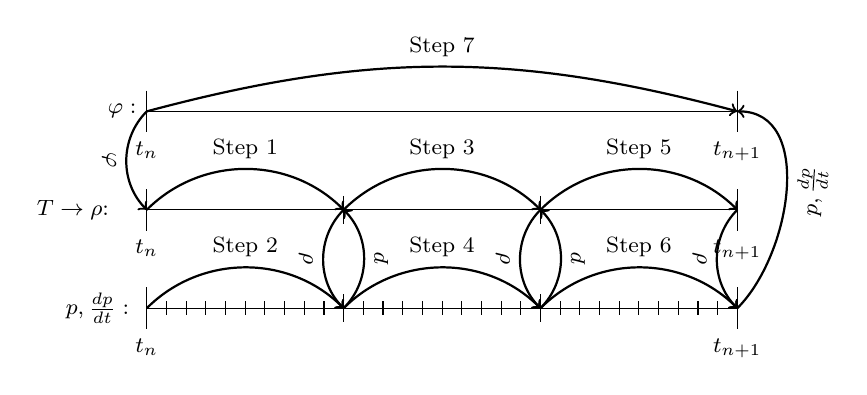
\begin{tikzpicture}[scale=1.25]
\tikzset{font={\footnotesize}}
%Shape
\draw[] (0,2) -- (6,2) ;
\foreach \x in  {0,6}
\draw[shift={(\x,2)},color=black] (0pt,6pt) -- (0pt,-6pt);
\draw[shift={(0,2)},color=black] (0pt,0pt) -- (0pt,-6pt) node[below] {$t_n$};
\draw[shift={(6,2)},color=black] (0pt,0pt) -- (0pt,-6pt) node[below] {$t_{n+1}$};
\node(shape) at (-.25,2) {$\varphi:$};

%Temp/Params
\draw[] (0,1) -- (6,1) ;
\foreach \x in  {0,6}
\draw[shift={(\x,1)},color=black] (0pt,6pt) -- (0pt,-6pt);
\foreach \x in  {2,4}
\draw[shift={(\x,1)},color=black] (0pt,4pt) -- (0pt,-4pt);
\draw[shift={(0,1)},color=black] (0pt,0pt) -- (0pt,-6pt) node[below] {$t_n$};
\draw[shift={(6,1)},color=black] (0pt,0pt) -- (0pt,-6pt) node[below] {$t_{n+1}$};
\node(temp) at (-.75,1) {$T \rightarrow \rho$:};

% PRKE
\draw[] (0,0) -- (6,0) ;
\foreach \x in  {0,6}
\draw[shift={(\x,0)},color=black] (0pt,6pt) -- (0pt,-6pt);
\foreach \x in  {0,2,4,6}
\draw[shift={(\x,0)},color=black] (0pt,4pt) -- (0pt,-4pt);
\foreach \x in  {0,0.2,0.4,0.6,0.8,1,1.2,1.4,1.6,1.8,2,2.2,2.4,2.6,2.8,3,3.2,3.4,3.6,3.8,4,4.2,4.4,4.6,4.8,5,5.2,5.4,5.6,5.8,6}
\draw[shift={(\x,0)},color=black] (0pt,2pt) -- (0pt,-2pt);
\draw[shift={(0,0)},color=black] (0pt,0pt) -- (0pt,-6pt) node[below] {$t_n$};
\draw[shift={(6,0)},color=black] (0pt,0pt) -- (0pt,-6pt) node[below] {$t_{n+1}$};
\node(prke) at (-.5,0) {$p, \frac{dp}{dt}:$};

\draw (0,0) edge[out=45,in=135,->,thick] node[above,sloped] {Step 2} (2,0);
\draw (2,0) edge[out=45,in=135,->,thick] node[above,sloped] {Step 4} (4,0);
\draw (4,0) edge[out=45,in=135,->,thick] node[above,sloped] {Step 6} (6,0);
\draw (0,1) edge[out=45,in=135,->,thick] node[above,sloped] {Step 1} (2,1);
\draw (2,1) edge[out=45,in=135,->,thick] node[above,sloped] {Step 3} (4,1);
\draw (4,1) edge[out=45,in=135,->,thick] node[above,sloped] {Step 5} (6,1);
\draw (0,2) edge[out=15,in=165,->,thick] node[above,sloped] {Step 7} (6,2);

\draw (0,2) edge[out=-135,in=135,->,thick] node[below,sloped] {$\varphi$} (0,1);
\draw (2,1) edge[out=-135,in=135,->,thick] node[below,sloped] {$\rho$} (2,0);
\draw (2,0) edge[out=45,in=-45,->,thick] node[below,sloped] {$p$} (2,1);
\draw (4,1) edge[out=-135,in=135,->,thick] node[below,sloped] {$\rho$} (4,0);
\draw (4,0) edge[out=45,in=-45,->,thick] node[below,sloped] {$p$} (4,1);
\draw (6,1) edge[out=-135,in=135,->,thick] node[below,sloped] {$\rho$} (6,0);
\draw (6,0) edge[out=45,in=0,->,thick] node[below,sloped] {$p, \frac{dp}{dt}$} (6,2);

\end{tikzpicture}
}
\end{figure}

\end{frame}
%-------------------------------------------------------------------

%-------------------------------------------------------------------
\begin{frame}{Time scale programming logic}

\begin{figure}
\centering
\resizebox{!}{3in}{
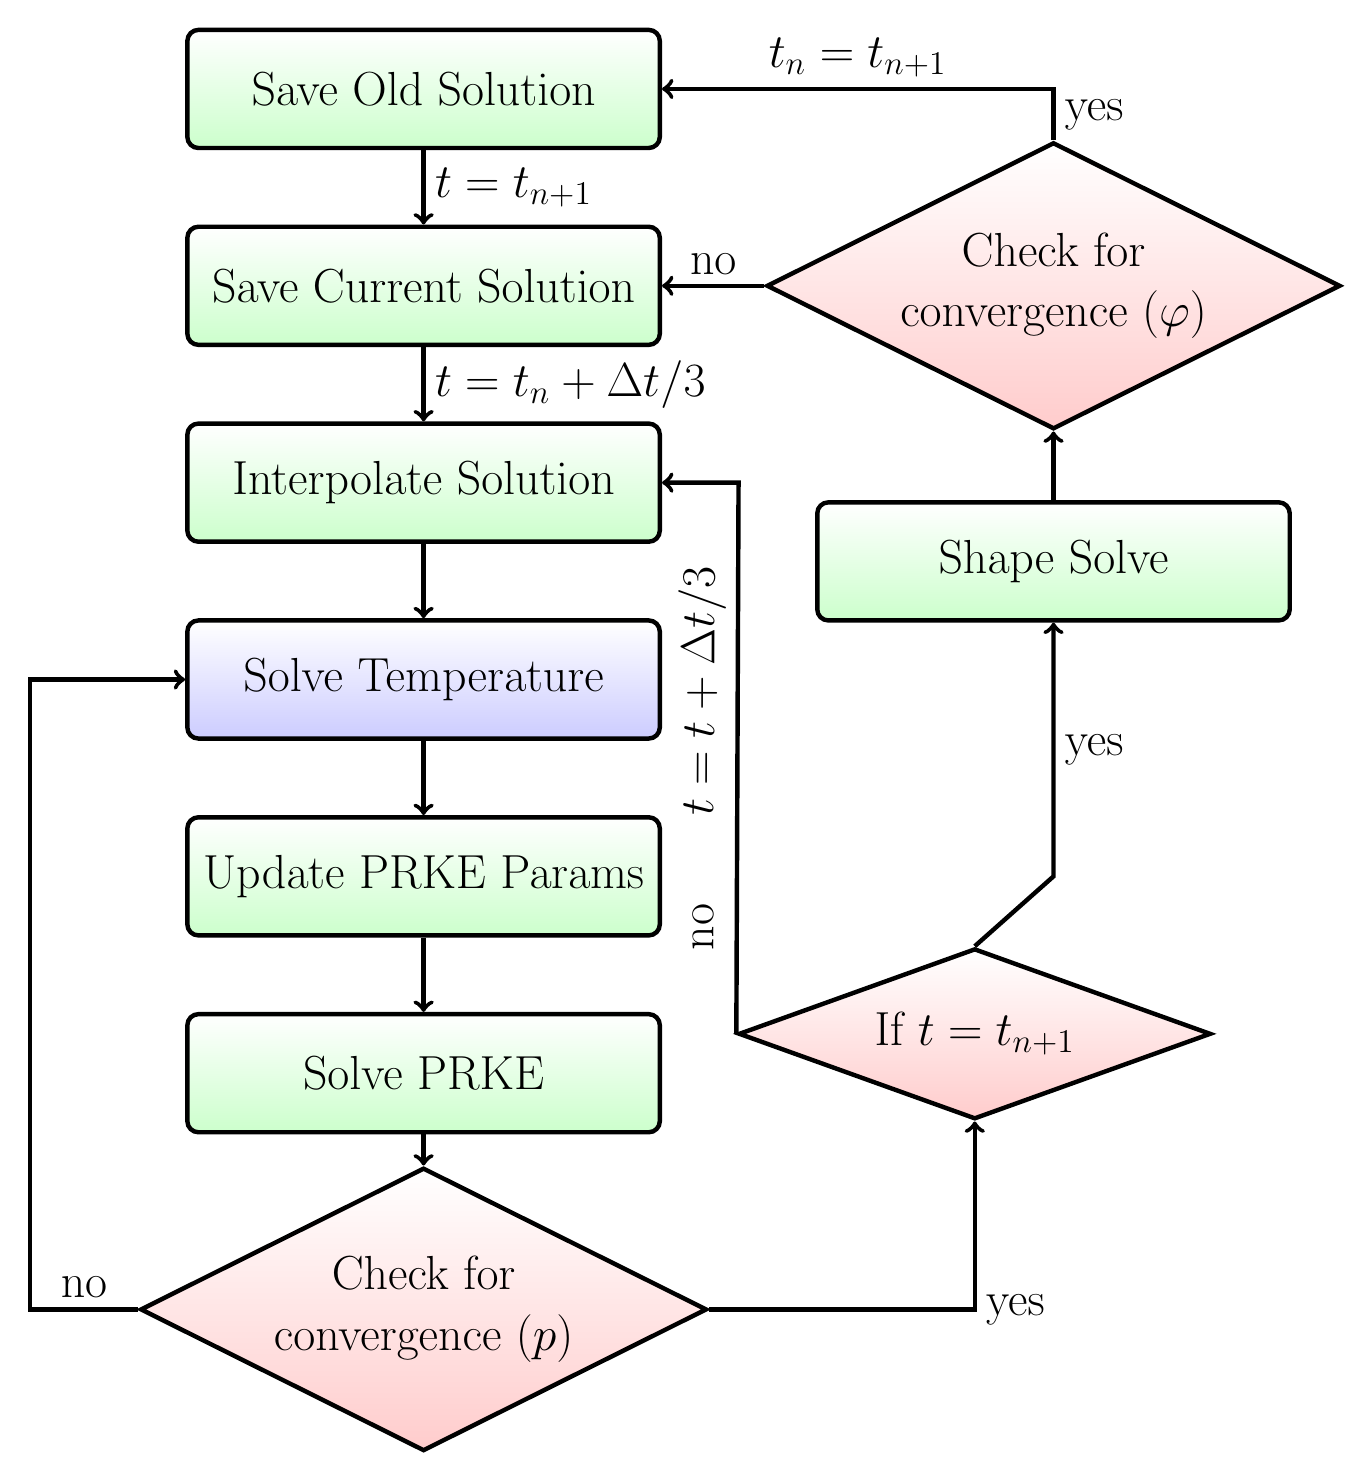
\begin{tikzpicture}[every node/.style = {font=\LARGE}]

\node[greenblock](p1) at (0,0) {Save Old Solution};
\node[greenblock](p2) at (0,-2.5) {Save Current Solution};
\node[greenblock](p3) at (0,-5) {Interpolate Solution};
\node[blueblock2](p4) at (0,-7.5) {Solve Temperature};
\node[greenblock] (p5) at (0,-10) {Update PRKE Params};
\node[greenblock] (p6) at (0,-12.5) {Solve PRKE};
\node[reddiamond] (check1) at (0,-15.5) {Check for \\ convergence ($p$)};
\node[reddiamond] (check2) at (7,-12) {If $t=t_{n+1}$};
\node[greenblock] (p7) at (8,-6) {Shape Solve};
\node[reddiamond] (check3) at (8,-2.5) {Check for \\ convergence ($\varphi$)};
%\node [above =0.1mm of p1] {\large{IQS Solve:}};
%\node [above =0.1mm of p5] {\large{Multi-physics:}};

%\tikzback{p1}{p1}{p4}{p4}{bk1}
%\tikzback{p5}{p5}{p5}{p5}{bk2}

\draw[->,ultra thick](p1.south) -- node[right] {$t=t_{n+1}$}(p2.north);
\draw[->,ultra thick](p2.south) -- node[right] {$t=t_{n}+\Delta t/3$}(p3.north);
\draw[->,ultra thick](p3.south) -- (p4.north);
\draw [->,ultra thick] (p4.south)-- (p5.north);
\draw[->,ultra thick](p5.south) -- (p6.north);
\draw[->,ultra thick](p6.south) -- (check1.north);
\draw[->,ultra thick](check1.west) -- node[above,sloped] {\LARGE{no}} (-5,-15.5) |-  (p4.west);
\draw[->,ultra thick](check1.east) -| node[right] {\LARGE{yes}} (check2.south);
\draw[->,ultra thick](check2.west) -- node[above,sloped] {\LARGE{no}\LARGE \qq $t=t+\Delta t/3$} (4,-5) -- (p3.east);
\draw[->,ultra thick](check2.north) --  (8,-10) -- node[right] {\LARGE{yes}} (p7.south);
\draw[->,ultra thick](p7.north) -- (check3.south);
\draw[->,ultra thick](check3.west) -- node[above] {no} (p2.east);
\draw[->,ultra thick](check3.north) -- node[right] {yes} (8,0) -- node[above] {$t_n=t_{n+1}$} (p1.east);

\end{tikzpicture}
}
\end{figure}

\end{frame}
%-------------------------------------------------------------------

%-------------------------------------------------------------------
\begin{frame}{Time Scale Analysis}

\begin{block}{Dynamical Time Scale}
\begin{itemize}
\item The time variance of each physics ($\theta$) can be quantified by defining a dynamical time scale ($\tau$):
\be
\tau = \frac{1}{\left|\frac{1}{\theta}\frac{d\theta}{dt}\right|}
\ee
\item Finite difference approximation for $d\theta/dt$ and average for $1/\theta$
\item Only temporal behavior is of interest, so the $L^2$ norm will be taken of each quantity, resulting in:
\be
\tilde{\tau}_{n+1} = \frac{\norm{\theta_{n+1} + \theta_{n}}}{2}\frac{\Delta t}{\norm{\theta_{n+1} - \theta_{n}}}
\ee
\item According to the a priori hypothesis, $\tau$ is large for \tcb{shape}, somewhat smaller for temperature, and much smaller for \tcr{amplitude} and flux
\end{itemize}
\end{block}

\end{frame}
%-------------------------------------------------------------------

\addtocontents{toc}{\newpage}
%%%%%%%%%%%%%%%%%%%%%%%%%%%%%%%%%%%%%%%%%%%%%%%%%%%%%%%%%%%%%%%%%%%%
\section{Implementation}
%%%%%%%%%%%%%%%%%%%%%%%%%%%%%%%%%%%%%%%%%%%%%%%%%%%%%%%%%%%%%%%%%%%%

%------------------------------------------------------------------%
\subsection{MOOSE/Rattlesnake}
%------------------------------------------------------------------%

%-------------------------------------------------------------------
\begin{frame}{Reactor Simulation in MOOSE}

\begin{figure}
\includegraphics[width=\linewidth]{figures/mammoth.png}
\end{figure}

\end{frame}
%-------------------------------------------------------------------

%%%%%%%%%%%%%%%%%%%%%%%%%%%%%%%%%%%%%%%%%%%%%%%%%%%%%%%%%%%%%%%%%%%%
\section{Results}
%%%%%%%%%%%%%%%%%%%%%%%%%%%%%%%%%%%%%%%%%%%%%%%%%%%%%%%%%%%%%%%%%%%%

%-------------------------------------------------------------------
\begin{frame}{Results}

\begin{multicols}{2}
\tableofcontents[currentsection]
\end{multicols}

\end{frame}
%-------------------------------------------------------------------

%------------------------------------------------------------------%
\subsection{LRA Benchmark}
%------------------------------------------------------------------%

%-------------------------------------------------------------------
\begin{frame}{LRA Benchmark}
\begin{columns}

\column{0.6\textwidth}
\begin{figure}
\includegraphics[width=\linewidth]{figures/lra.png}
\end{figure}

\column{0.6\textwidth}
\begin{figure}
\includegraphics[width=\linewidth]{figures/lra_profile2D.png}
\end{figure}

\end{columns}
\end{frame}
%-------------------------------------------------------------------

%-------------------------------------------------------------------
\begin{frame}{LRA Power and Temperature Profile}

\begin{figure}
\includegraphics[width=\linewidth,height=3in,keepaspectratio]{figures/lra_profile.png}
\end{figure}

\end{frame}
%-------------------------------------------------------------------

%-------------------------------------------------------------------
\begin{frame}{LRA Time Step Error Convergence}
\begin{columns}

\column{0.6\textwidth}
\begin{figure}
\includegraphics[width=\linewidth]{figures/lra_bad.png}
\caption{Only one temperature update per macro step}
\end{figure}

\column{0.6\textwidth}
\begin{figure}
\includegraphics[width=\linewidth]{figures/lra_mp_convergence.png}
\caption{Five temperature updates per macro step}
\end{figure}

\end{columns}
\end{frame}
%-------------------------------------------------------------------

%-------------------------------------------------------------------
\begin{frame}{Analysis on Temperature Updates}

\begin{columns}

\column{.6\textwidth}
\begin{figure}
\includegraphics[width=\textwidth]{figures/lra_mp.png}
\end{figure}

\column{.5\textwidth}
\vspace{-5mm}
\begin{table}
\captionsetup{font=scriptsize}
\begin{center}
\colorbox{white}{\resizebox{\textwidth}{!}{
\begin{tabular}{|l|l|ccc|}
\hline
\multicolumn{5}{|c|}{Implicit Discretization}\\
\hline
Run  &  $\Delta t$ & Error & Runtime (hr) & Linear Iter.\\
\hline
1	& 4.0e-3	& 1.407e-2 	& 4.11	& 7.13e4	\\
\hline
\rowcolor{yellow} 2	& 2.0e-3	& 3.174e-3 	& 6.01	& 9.49e4 	\\
\hline
\rowcolor{green} 3 	& 1.0e-3 	& 7.690e-4 	& 10.38	& 1.45e5	\\
\hline
4 	& 5.0e-4 	& 1.892e-4 	& 21.91	& 2.08e5	\\
5 	& 2.5e-4	& 4.590e-5 	& 25.23	& 3.16e5	\\
\hline
\end{tabular}}}
\end{center}
\end{table}
\vspace{-7mm}

\begin{table}
\captionsetup{font=small}
\begin{center}
\colorbox{white}{\resizebox{\textwidth}{!}{
\begin{tabular}{|l|l|ccc|}
\hline
\multicolumn{5}{|c|}{IQS}\\
\hline
	&  Temperature 	&  		& Runtime 	& \% Increase	\\
Run	&  Updates 	& Error & (hr)		& in Runtime$^*$\\
\hline
\rowcolor{yellow} 1	& 1		& 2.612e-3 	& 3.96 	& -3.18\%	\\
\hline
2	& 2		& 9.893e-4 	& 6.02	&  47.1\%	\\
3 	& 4 	& 5.796e-4 	& 7.87	&  92.3\%	\\
4 	& 8 	& 4.772e-4 	& 12.61	& 207.9\% 	\\
5 	& 16	& 4.516e-4 	& 22.14	& 440.7\%	\\
\hline
\end{tabular}}}
\end{center}
\end{table}
\vspace{-7mm}

\begin{table}
\captionsetup{font=scriptsize}
\begin{center}
\colorbox{white}{\resizebox{\textwidth}{!}{
\begin{tabular}{|l|l|ccc|}
\hline
\multicolumn{5}{|c|}{IQS P-C}\\
\hline
	&  Temperature 	&  		& Runtime 	& \% Increase	\\
Run	&  Updates 	& Error & (hr)		& in Runtime$^*$\\
\hline
1	& 1		& 3.488e-3 	& 2.91 	& -28.9\%	\\
2	& 2		& 1.349e-3 	& 3.73	& -9.00\%	\\
\hline
\rowcolor{green} 3 	& 4 	& 9.161e-4 	& 3.97	& -3.04\%	\\
\hline
4 	& 8 	& 8.052e-4 	& 5.39	&  31.7\%	\\
5 	& 16	& 7.905e-4 	& 8.19	&  100\%	\\
\hline
\end{tabular}}}
%}
\\
\tiny $^*$ runtime difference from $\Delta t = 0.004$ implicit dis.
\end{center}
\end{table}

\end{columns}

\end{frame}
%-------------------------------------------------------------------

%-------------------------------------------------------------------
\begin{frame}{LRA Dynamical Time Scale Analysis}

\begin{figure}
\includegraphics[width=\linewidth,height=3in,keepaspectratio]{figures/time_constant_lra.png}
\end{figure}

\end{frame}
%-------------------------------------------------------------------

%------------------------------------------------------------------%
\subsection{TREAT Transient-15}
%------------------------------------------------------------------%

%-------------------------------------------------------------------
\begin{frame}{TREAT: Transient-15 Example}
\begin{columns}

\column{0.6\textwidth}
\begin{figure}
\includegraphics[width=\linewidth]{figures/Tran15_config.png}
\end{figure}

\column{0.5\textwidth}
\begin{figure}
\includegraphics[width=\linewidth]{figures/Tran15_mesh_homo.png}
\end{figure}

\end{columns}
\end{frame}
%-------------------------------------------------------------------

%-------------------------------------------------------------------
\begin{frame}{Transient-15 Power Profile}
\begin{columns}

\column{0.6\textwidth}
\begin{figure}
\includegraphics[width=\linewidth]{figures/Tran15_core2.png}
\end{figure}

\column{0.5\textwidth}
\begin{figure}
\includegraphics[width=\linewidth]{figures/Tran15_profile.png}
\end{figure}

\end{columns}
\end{frame}
%-------------------------------------------------------------------

%-------------------------------------------------------------------
\begin{frame}{Transient-15 Results}
\vspace{-3mm}

\begin{block}{Accuracy and Runtime}
\begin{center}
\resizebox{\linewidth}{!}{
\begin{tabular}{|l|ccc|}
\hline
Method & No. of Steps & \% Increase Runtime$^*$ & Max Power Error \\
\hline
Implicit Dis. 		& 300 &	---		&	7.875e-4	\\
\hline
\rowcolor{yellow} IQS 				& 300 & -11.9\%	&	8.385e-5	\\
\hline
IQS (5 updates) 	& 300 &  49.7\%	&	3.687e-5	\\
IQS P-C 			& 300 &  -2.1\%	&	7.527e-4	\\
\hline
\rowcolor{green} IQS P-C (5 updates) & 300 &  26.5\%	&	1.227e-4	\\
\hline
\end{tabular}
}
\end{center}
\vspace{-3mm}
$^*$ difference in runtime from implicit discretization 
\end{block}

\begin{block}{Dynamical Time Scale}
\begin{figure}
\includegraphics[height=1.5in]{figures/time_constant_tran15.png}
\end{figure}
\end{block}


\end{frame}
%-------------------------------------------------------------------

%%%%%%%%%%%%%%%%%%%%%%%%%%%%%%%%%%%%%%%%%%%%%%%%%%%%%%%%%%%%%%%%%%%%
\section{Conclusions}
%%%%%%%%%%%%%%%%%%%%%%%%%%%%%%%%%%%%%%%%%%%%%%%%%%%%%%%%%%%%%%%%%%%%

%-------------------------------------------------------------------
\begin{frame}{Conclusions}
\vspace{-3mm}

\begin{block}{Summary}
\begin{itemize}
\item Derivation of IQS and implementation of quasi-static time stepping
\item Semi-analytic evaluation of temperature
\item Implementation of adiabatic heat up in quasi-static process
\item Testing with LRA benchmark and TREAT Transient-15 model
\end{itemize}
\end{block}

\begin{block}{Conclusions}
\begin{itemize}
\item Temperature-amplitude iteration decreased temperature-shape iteration
\item Semi-analytic temperature evaluation improved IQS CPU performance
\item Intermediate time scale significantly improved IQS time step performance.
\item Optimal CPU performance with 1 update for IQS and 4 updates for IQS P-C
\item Time constant analysis showed adaptation could further improve performance
\end{itemize}
\end{block}

\begin{block}{Future Work}
\begin{itemize}
\item Implement intermediate time scale to more advanced multiphysics
\item Develop adaptation technique for number of multipysics updates
\end{itemize}
\end{block}

\end{frame}
%-------------------------------------------------------------------

%-------------------------------------------------------------------
\begin{frame}{Questions?}

\centering
\includegraphics[width=\linewidth,height=3in,keepaspectratio]{figures/question_mark.jpg}

\end{frame}
%-------------------------------------------------------------------

%-------------------------------------------------------------------
\begin{frame}{Acknowledgments}

\begin{block}{}
\begin{itemize}
\item This material is based upon work supported under an Integrated University Program Graduate Fellowship
\begin{figure}
\includegraphics[height=0.5in]{figures/IUP_Logo.jpeg}
\end{figure}
\item Any opinions, findings, conclusions or recommendations expressed in this publication are those of the author(s) and do not necessarily reflect the views of the Department of Energy Office of Nuclear Energy
\end{itemize}
\end{block}

\begin{figure}
\includegraphics[height=0.5in]{figures/tamune_logo.png}
\end{figure}
\begin{figure}
\includegraphics[height=0.5in]{figures/INL_logo.png}
\end{figure}

\end{frame}
%-------------------------------------------------------------------

%%%%%%%%%%%%%%%%%%%%%%%%%%%%%%%%%%%%%%%%%%%%%%%%%%%%%%%%%%%%%%%%%%%%
\backupbegin
%%%%%%%%%%%%%%%%%%%%%%%%%%%%%%%%%%%%%%%%%%%%%%%%%%%%%%%%%%%%%%%%%%%%

%-------------------------------------------------------------------
\begin{frame}{Rattlesnake Structure}

\begin{figure}
\includegraphics[width=\linewidth,height=\textheight,keepaspectratio]{figures/rattlesnake.png}
\end{figure}

\end{frame}
%-------------------------------------------------------------------

%-------------------------------------------------------------------
\begin{frame}{IQS Implementation in Rattlesnake}

\begin{block}{IQS Components in Rattlesnake}
\begin{itemize}
\item IQS Executioner
	\begin{itemize}
	\item Convergence criteria for Picard iteration:
	\be
	Error_{IQS}=\left|\frac{\sum_{g=1}^G\left(\phi^{*g},\frac{1}{v^g}\varphi^{g,n}\right)}{\sum_{g=1}^G\left(\phi^{*g},\frac{1}{v^g}\varphi^{g,0}\right)}-1\right|
	\ee
	\item Evaluates PRKE using implicit Euler, Crank-Nicolson, or SDIRK33 with step doubling adaptation for $\frac{1}{p}\frac{dp}{dt}$ term
	\end{itemize}
\item PRKE Parameter Postprocessors
	\begin{itemize}
	\item Performs integrations for PRKE parameters
	\item Residuals from kernels are saved for $\rho-\bar{\beta}$ integration
	\end{itemize}
\item PRKE User Object
	\begin{itemize}
	\item Gathers postprocessor values
	\end{itemize}
\item IQS Removal Kernel
	\begin{itemize}
	\item Removal kernel for $\frac{1}{v^g}\frac{1}{p}\frac{dp}{dt}\varphi^g$ term
	\end{itemize}
\item Auxkernels
	\begin{itemize}
	\item Precursor auxkernel with analytical integration
	\item Temperature auxkernel with analytical integration
	\end{itemize}
\end{itemize}
\end{block}

\end{frame}
%-------------------------------------------------------------------

%-------------------------------------------------------------------
\begin{frame}{IQS Implementation in Rattlesnake (cont.)}
\vspace{-3mm}
\begin{block}{IQS Kernels}
\small
\begin{align*}
\frac{1}{v^g}\frac{\partial\varphi^g}{\partial t}=&\underbrace{\frac{\chi_p^g}{\keff} \sum_{g'=1}^G (1-\beta) \nu^{g'} \Sigma_f^{g'} \varphi^{g'}}_{Flux Kernel} + \underbrace{\sum_{g'\neq g}^G\Sigma_s^{g'\to g} \varphi^{g'}}_{Flux Kernel} - \underbrace{\left( -\div D^g \grad \right)\varphi^g}_{Flux Kernel} - \underbrace{\Sigma_r^g\varphi^g}_{Flux Kernel} \nonumber \\
& - \underbrace{\frac{1}{v^g} \boxed{\overbrace{\frac{1}{p}\frac{dp}{dt}}^{From Executioner}}\varphi^g}_{IQS Kernel}+\underbrace{\frac{1}{p}\sum_{i=1}^I\chi_{d,i}^g\lambda_iC_i}_{Modified Flux Kernel}
\end{align*}
\end{block}
\vspace{-2mm}

\begin{figure}
\resizebox{!}{1.5in}{
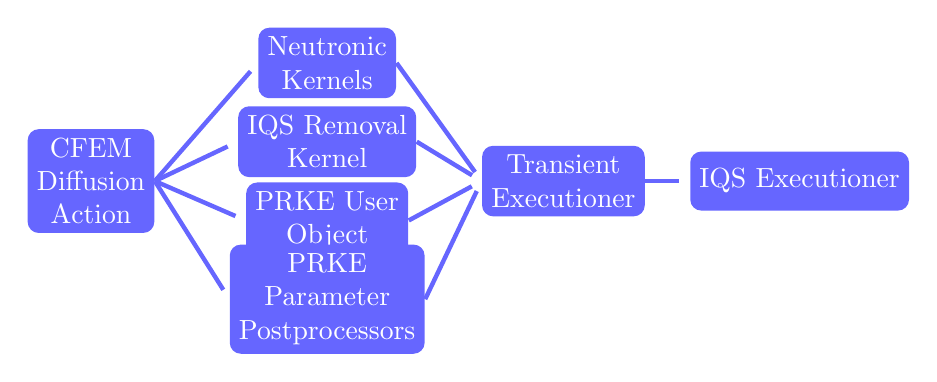
\begin{tikzpicture}[every node/.style = {shape          = rectangle, rounded corners, fill = blue!60, minimum width  = 1.5cm, minimum height = 0.75cm, align= center, text = white},blue edge/.style  = { -, ultra thick, blue!60, shorten >= 4pt}]
\node(0;0) at (-1,0) {CFEM \\ Diffusion \\ Action};
  \node(1;3)  at (2, 1.5) {Neutronic \\ Kernels};   
  \node(1;1)  at (2, 0.5) {IQS Removal \\ Kernel}; 
  \node(1;-1)  at (2,-0.5) {PRKE User \\ Object}; 
  \node(1;-3) at (2,-1.5) {PRKE \\ Parameter \\ Postprocessors}; 
     \node(2;0)  at (5,0) {Transient \\ Executioner};
     	\node(3;0)  at (8,0) {IQS Executioner};
\foreach \j in {-3,-1,1,3}
  { \draw[blue edge] (0;0.east) -- (1;\j.west); }
\foreach \j in {-3,-1,1,3}
  { \draw[blue edge] (1;\j.east) -- (2;0.west);} 
\draw[blue edge] (2;0.east) -- (3;0.west);         
\end{tikzpicture}
}
\end{figure}

\end{frame}
%-------------------------------------------------------------------

%%%%%%%%%%%%%%%%%%%%%%%%%%%%%%%%%%%%%%%%%%%%%%%%%%%%%%%%%%%%%%%%%%%%
\backupend
%%%%%%%%%%%%%%%%%%%%%%%%%%%%%%%%%%%%%%%%%%%%%%%%%%%%%%%%%%%%%%%%%%%%

%************************************************

\end{document}